\chapter{The Physical Layer}
\label{cha:physicallayer}

\section{Overview}

TODO: motivation in general? radio frames shared transmission, immutable data structures?

In the field of communication system simulations one of the most time consuming
task is to simulate the physical layer. The simulation of transmissions, receptions
and interferences in detail may often result in unacceptable performance. Finding
the right abstractions, the right level of detail is difficult and very important.

The physical layer in INET was designed with the following goals in mind:
\begin{itemize}
  \item customizability
  \item extensibility
  \item scalable level of detail
  \item ability to exploit parallel hardware
\end{itemize}

This chapter provides a brief overview of the physical layer model. For more
details on the available modules, their parameterization and the actual
implementations please refer to the documentation in the corresponding NED and
C++ source files.

\subsection{Customizability}

The physical layer provides a wide variety of parameters to control its behavior.
The most common parameters are physical quantities with physical units such as
transmission power \ttt{[W]}, reception sensitivity \ttt{[W]}, carrier frequency
\ttt{[Hz]}, propagation speed \ttt{[m/s]}, SNIR threshold \ttt{[dB]}, communication
range \ttt{[m]}, bitrate \ttt{[b/s]}, etc. 

Another commonly used parameter kind is the one that selects among alternative
implementations by providing its name. Different implementations are separate
modules that come with their own set of parameters to avoid the confusion of
mixing unrelated parameters. Some modules may be split into more submodules 
further deepening the module hierarchy.

\subsection{Extensibility}

The physical layer is designed to be extensible with alternative implementations
for various parts of the model. This is realized by separately defining C++ and
NED interfaces between modules, and also by providing parameters in their parent
modules to easily select among the available implementations.

New models can be added by implementing the necessary interfaces with optionally
deriving from already existing ones. This allows the user to implement new models
with less effort and focus on the real differences while the rest of the physical
layer model remains the same.

\subsection{Scalable Level of Detail}

The physical layer is designed to be scalable with respect to the simulated level
of detail. There are many possible ways to model various physical layer aspects.
The main difference lies in the trade-off between performance versus accuracy.

The model might vary from simple statistical to accurate emulation. The simplest
models ignore actual bits or even signal power for that matter. The most accurate
models use bit precise signal representation and emulate most functions of real
hardware in detail.

The software architecture might vary from flat to layered. A flat architecture
is efficient but not modular. Functionality can only be affected through simple
parameters and not by providing alternative implementations. Whereas a layered
architecture is more flexible at the cost of more complex data structures, more
data conversions, more resource management, and thus slower processing. On the
other hand, it provides more customization opportunities to replace parts with
alternative implementations and do research in this area.

The data representation might vary from scalar to multidimensional values. In
the physical layer data quite often changes over time, frequency, space, or any
combination thereof. The most obvious example is the analog signal power but 
there are others such as signal phase, bitrate or the signal to noise ratio.

The number of messages added to the future event queue might vary from one to
the number of radios per transmission. One message might be sufficient for example,
if the transmission is intended to a single destination and other receivers are
either not affected or the effect is negligible with respect to accuracy. On the
other hand, sometimes it might be necessary to process all transmissions by all
receivers in order to have the desired effect on higher layers.

\subsection{Exploiting Parallel Hardware}

The physical layer is designed to utilize parallel hardware, multi-core CPUs,
vector instructions and the highly parallel GPU. The computation of transmission
arrival space-time coordinates, receptions, interferences, reception indications
provide a good parallelization opportunity, because they dominate the physical
layer performance and are independent of each other. 

The medium module is a central component in the software architecture where
parallel computation can happen. One possibility is optimistic parallel
computation of results in multiple background threads while the main simulation
thread continues normal execution. As new transmissions enter the channel the
affected and already computed results are invalidated and the affected ongoing
optimistic parallel computations are canceled.

\section{The Radio Module}

The radio module represents the physical device that is capable of transmitting
and receiving signals on the medium. It consists of an antenna, a transmitter, a
receiver and a power consumer model. It supports the following externally
configurable radio modes: 

\begin{itemize}
  \item \ttt{off}: communication isn't possible and power consumption is zero
  \item \ttt{sleep}: communication isn't possible and power consumption is minimal
  \item \ttt{receiver}: only reception is possible and power consumption is low
  \item \ttt{transmitter}: only transmission is possible and power consumption
is high
  \item \ttt{transceiver}: reception and transmission is simultaneously possible
and power consumption is high
  \item \ttt{switching}: communication isn't possible and power consumption is
minimal
\end{itemize}

The radio module also supports non-zero time radio mode switching. In addition,
the transmitter and the receiver parts have separate states which describe what
they are doing at the moment. Changes to these states are automatically published
by the radio.

When the radio wants to transmit a signal on the medium it sends direct messages
to other radios with the help of the central medium module. Receiver radios also
handle the incoming messages with the help by the central medium module.

The radio module utilizes multiple submodules to further split its task. This
design makes it extensible and customizable. The following sections describe the
parts of the radio.

\subsection{Antenna Models}

The antenna models represent the physical device which converts electric signals
into radio waves, and vice versa. They provide position and orientation using a
mobility model that defaults to the mobility of the radio. They also compute the
antenna gain based on antenna characteristics and the position and the orientation
of the transmitter and the receiver. The following list provides some examples:

\begin{itemize}
  \item \nedtype{IsotropicAntenna}: antenna gain is exactly 1 in any direction
  \item \nedtype{ConstantGainAntenna}: antenna gain is a constant determined by
a parameter
  \item \nedtype{DipoleAntenna}: antenna gain depends on the direction according
to the dipole antenna characteristics
  \item \nedtype{InterpolatingAntenna}: antenna gain is computed by a linear
interpolation according to a table index by the direction angles
\end{itemize}

The antenna models are in the \ttt{src/physicallayer/antenna/} directory.

\subsection{Transmitter Models}

This module represents the physical device which converts packets into electric
signals. It takes a MAC frame and produces a description of the signal that is
transmitted on the medium.

TODO

\subsection{Receiver Models}

This module represents the physical device which converts electric signals into
packets. It takes a signal along with the interference computed by the medium
and it produces a MAC frame along with a reception indication.

TODO

\subsection{Error Models}

TODO

\subsection{Power Consumer Models}

TODO: hivatkozas a power model-re?

The power consumer models describe how the radio consumes power depending on the
operational mode, the transmitted and the received signals. The following list
provides some examples:

\begin{itemize}
  \item \nedtype{SimplePowerConsumer}: power consumption is determined by the
radio mode, the transmitter state and the receiver state
\end{itemize}

The power consumer models are in the \ttt{src/physicallayer/power/} directory.

\iffalse TODO: implementation incomplete
\subsection{Layered Radio Model}

This module further splits the transmitter and receiver models to allow bit
precise communication modeling.

TODO

The following sections describe the parts of the layered radio model.

\subsubsection{Encoding and Decoding}

This module describes how the packet domain signal representation is converted
into the bit domain, and vice versa.

TODO

\subsubsection{Modulation and Demodulation}

This module describes how the bit domain signal representation is converted into
the symbol domain, and vice versa.

TODO

\subsubsection{Pulse Shaping and Pulse Filtering}

This module describes how the symbol domain signal representation is converted
into the sample domain, and vice versa.

TODO

\subsubsection{Digital Analog and Analog Digital Conversion}

This module describes how the sample domain signal representation is converted
into the analog domain, and vice versa.

TODO
\fi

\section{The Medium Module}

The medium module represents the shared physical medium where communication
takes place. It keeps track of radios, noise sources, ongoing transmissions,
background and other noises. The medium computes when, where and how
transmissions and noises arrive at receivers. It also efficiently provides the
set of interfering transmissions and noises for the receiver to compute the
reception indication. It doesn't send or handle messages on its own, but it
rather acts as a mediator between radios.

The medium module utilizes multiple submodules to further split its task. This
design  makes it extensible and customizable. The following sections describe
the parts of the medium.

\subsection{Propagation Models}

TODO: difficulty, motivation? with respect to transmitter and receiver mobility

The propagation models are separate modules which describe how signals propagate
through space over time. They compute the arrival space-time coordinates for
transmissions. The following list provides some examples:

\begin{itemize}
  \item \nedtype{ConstantTimePropagation}: propagation time is independent of
  the traveled distance and it's determined by a constant parameter
  \item \nedtype{ConstantSpeedPropagation}: propagation time is proportional to
  the traveled distance determined by a constant propagation speed parameter
  \item \nedtype{ConstantSpeedGPUPropagation}: propagation time is computed in
  parallel on the GPU for all receivers
\end{itemize}

The propagation models are in the \ttt{src/physicallayer/propagation/} directory.

\subsection{Path Loss Models}

TODO: difficulty, motivation?

The path loss models are separate modules which describe the reduction of power
as the signal propagates through space. They compute the power loss factor based
on the traveled distance, the signal frequency and the propagation speed. They
may also provide the opposite, that is the traveled distance based on the power
loss factor, the signal frequency and the propagation speed. The following list
provides some examples:

\begin{itemize}
  \item \nedtype{FreeSpacePathLoss}
  \item \nedtype{LogNormalShadowing}
  \item \nedtype{TwoRayGroundReflection}
  \item \nedtype{BreakpointPathLoss}
  \item \nedtype{NakagamiFading}
  \item \nedtype{RayleighFading}
  \item \nedtype{RicianFading}
  \item \nedtype{SUIPathLoss}
  \item \nedtype{UWBIRStochasticPathLoss}
  \item etc.
\end{itemize}

The path loss models are in the \ttt{src/physicallayer/pathloss/} directory.

\subsection{Obstacle Loss Models}

TODO: hivatkozas a physical environment modelre?

The obstacle loss models describe the reduction of power as the signal propagates
through obstacles. They compute the power loss factor based on the traveled straight
path, the signal frequency and the obstructing physical objects. The following list
provides some examples:

\begin{itemize}
  \item \nedtype{TracingObstacleLoss}: the power loss is based on accurate
dielectric and reflection loss along the straight path considering the shape,
position, orientation and material of physical objects
\end{itemize}

The obstacle loss models are in the \ttt{src/physicallayer/obstacleloss/} directory.

\iffalse TODO: implementation incomplete
\subsection{Multipath Models}

The multipath models describe the alternative paths that the signal travels before
it either reaches the receiver or sufficiently fades.

TODO
\fi

\subsection{Background Noise Models}

The background noise models describe how the background noise changes over space
and time. They compute the noise signal for a given space-time interval.

\begin{itemize}
  \item \nedtype{IsotropicBackgroundNoise}: the noise is independent of time and
position and its power is determined by a constant parameter 
\end{itemize}

The background noise models are in the \ttt{src/physicallayer/backgroundnoise/}
directory.

\subsection{Neighbor Cache Models}

The neighbor cache models provide an efficient way of keeping track of the neighbor
relationship between radios. They maintain the potential set of receivers for all
transmitters on the medium. They follow radio position changes but may provide
conservative approximations. The following list provides some examples:

\begin{itemize}
  \item \nedtype{ListNeighborCache}: maintains a separate periodically updated 
neighbor list for each radio
  \item \nedtype{GridNeighborCache}: organizes radios in a 3 dimensional grid
with constant cell size and updates periodically
  \item \nedtype{QuadTreeNeighborCache}: organizes radios in a 2 dimensional
quad tree (ignoring the Z axis) with constant node size and updates periodically
\end{itemize}

The neighbor cache models are in the \ttt{src/physicallayer/neighborcache/}
directory.

\section{Signal Representations}

TODO

\subsection{Flat Representation}

TODO

\begin{center}
\begin{figure}
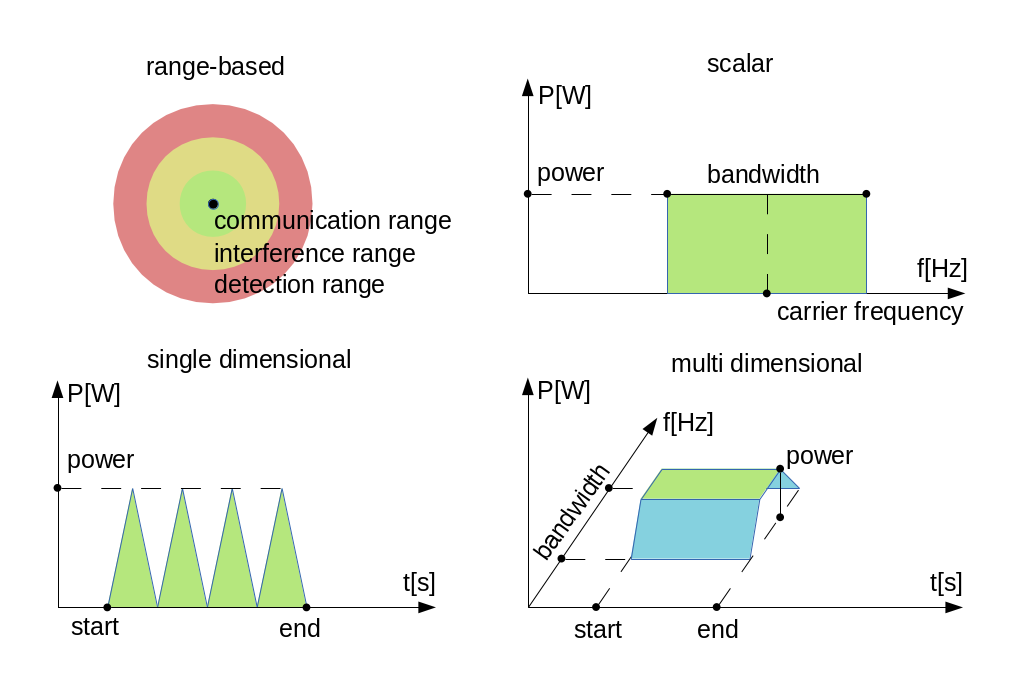
\includegraphics[width=\textwidth]{figures/phyanalog}
\caption{Analog signal representations}
\end{figure}
\end{center}

\subsection{Layered Representation}

TODO

\subsubsection{Packet Domain}

TODO

\subsubsection{Bit Domain}

TODO

\subsubsection{Symbol Domain}

TODO

\subsubsection{Sample Domain}

TODO

\subsubsection{Analog Domain}

TODO

\section{Signal Processing}

TODO

\begin{center}
\begin{figure}
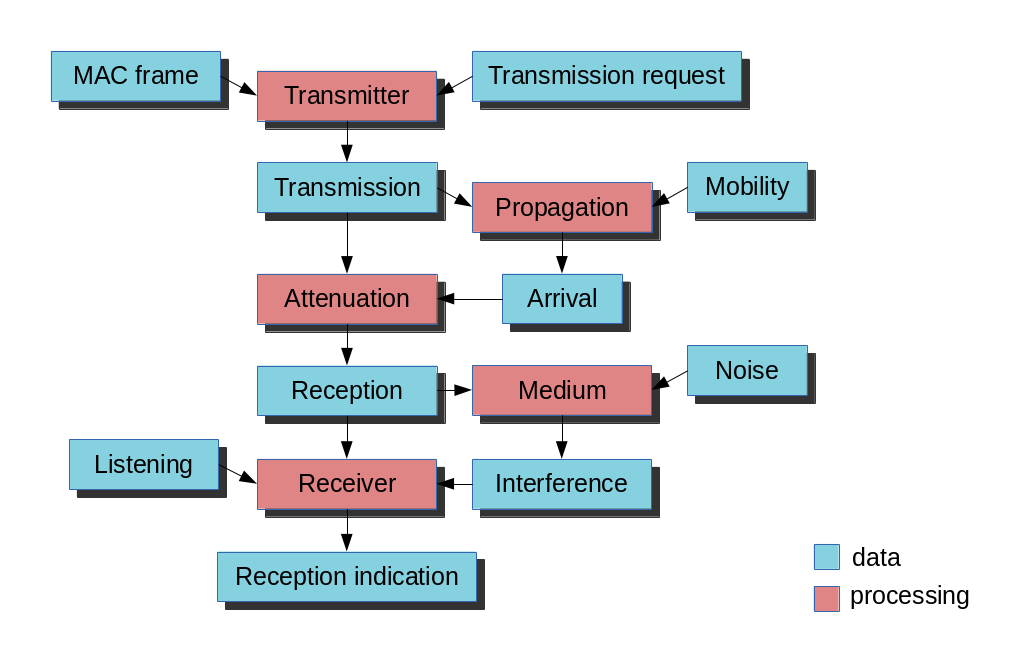
\includegraphics[width=\textwidth]{figures/phydataflow}
\caption{Data flow}
\end{figure}
\end{center}

The following sections describe the data structures of the data flow.

\subsection{Transmission Request}

This data structure contains parameters that control how the transmitter produces
the transmission. It is attached as a control info object to the MAC frame sent
down from the MAC module to the radio.

\subsection{Transmission}

This data structure represents the transmission of a radio signal. All models
contain at least the start/end time, start/end antenna position, start/end antenna
orientation of the transmitter.

\subsection{Arrival}

This data structure contains information about the space and time coordinates of
a transmission arriving at a particular receiver. It contains at least the 
start/end time, start/end antenna position, start/end antenna orientation of the
receiver. 

\subsection{Listening}

TODO

\subsection{Reception}

This data structure represents the reception of a radio signal by a particular
receiver. All models contain at least the start/end time, start/end antenna position,
start/end antenna orientation of the receiver. 

\subsection{Interference}

TODO

\subsection{Reception Decision}

TODO

\subsection{Reception Indication}

TODO

\section{Visualization}

The physical layer provides some parameters to display various internal state
such as ongoing transmissions, recent successful receptions and recent obstacle
intersections.

%%% Local Variables:
%%% mode: latex
%%% TeX-master: "usman"
%%% End:

